\documentclass[11pt,a4paper]{report}

% ============================================================================
% PACKAGES
% ============================================================================
\usepackage[utf8]{inputenc}
\usepackage[T1]{fontenc}
\usepackage{helvet}
\renewcommand{\familydefault}{\sfdefault}
\usepackage[margin=2.5cm, headheight=25pt]{geometry}
\usepackage{xcolor}
\usepackage{colortbl}
\usepackage{booktabs}
\usepackage{tabularx}
\usepackage{array}
\usepackage{graphicx}
\usepackage{tikz}
\usepackage{fancyhdr}
\usepackage{enumitem}
\usepackage{multirow}
\usepackage{calc}
\usepackage{amssymb}
\usepackage{pifont}
\usepackage{titlesec}
\usepackage{tocloft}
\usepackage[hidelinks]{hyperref}
\usetikzlibrary{shapes.geometric, arrows, positioning, calc, patterns}

% ============================================================================
% COLOR DEFINITIONS
% ============================================================================
\definecolor{miloprimary}{RGB}{37, 99, 235}
\definecolor{milosecondary}{RGB}{99, 102, 241}
\definecolor{miloaccent}{RGB}{14, 165, 233}
\definecolor{freegray}{RGB}{107, 114, 128}
\definecolor{bronzecolor}{RGB}{205, 127, 50}
\definecolor{silvercolor}{RGB}{156, 163, 175}
\definecolor{goldcolor}{RGB}{234, 179, 8}
\definecolor{platinumcolor}{RGB}{139, 92, 246}
\definecolor{successgreen}{RGB}{34, 197, 94}
\definecolor{warningorange}{RGB}{249, 115, 22}
\definecolor{dangerred}{RGB}{239, 68, 68}
\definecolor{lightbg}{RGB}{248, 250, 252}
\definecolor{darktext}{RGB}{30, 41, 59}
\definecolor{infoblue}{RGB}{59, 130, 246}
\definecolor{darkgreen}{RGB}{22, 163, 74}
\definecolor{appstoreblue}{RGB}{0, 122, 255}
\definecolor{datapurple}{RGB}{139, 92, 246}
\definecolor{analyticsteal}{RGB}{20, 184, 166}
\definecolor{competitorblue}{RGB}{59, 130, 246}

% ============================================================================
% HYPERREF SETUP
% ============================================================================
\hypersetup{
    colorlinks=true,
    linkcolor=miloprimary,
    urlcolor=miloprimary,
    pdftitle={MILO Business Report V3 - Seed Funding},
    pdfauthor={DeepmAInd B.V.}
}

% ============================================================================
% HEADER/FOOTER CONFIGURATION
% ============================================================================
\pagestyle{fancy}
\fancyhf{}
\fancyhead[L]{\textcolor{miloprimary}{\textbf{MILO}}}
\fancyhead[R]{\textcolor{freegray}{Seed Funding Report V3}}
\fancyfoot[C]{\textcolor{freegray}{\thepage}}
\renewcommand{\headrulewidth}{2pt}
\renewcommand{\headrule}{\hbox to\headwidth{\color{miloprimary}\leaders\hrule height \headrulewidth\hfill}}

% ============================================================================
% CHAPTER/SECTION FORMATTING
% ============================================================================
\titleformat{\chapter}[display]
{\normalfont\huge\bfseries\color{miloprimary}}
{\chaptertitlename\ \thechapter}{20pt}{\Huge}
\titlespacing*{\chapter}{0pt}{-30pt}{30pt}

\titleformat{\section}
{\normalfont\Large\bfseries\color{miloprimary}}
{\thesection}{1em}{}

\titleformat{\subsection}
{\normalfont\large\bfseries\color{milosecondary}}
{\thesubsection}{1em}{}

% ============================================================================
% TABLE OF CONTENTS FORMATTING
% ============================================================================
\renewcommand{\cftchapfont}{\bfseries\color{miloprimary}}
\renewcommand{\cftsecfont}{\color{darktext}}
\renewcommand{\cftsubsecfont}{\color{freegray}}
\renewcommand{\cftchapleader}{\cftdotfill{\cftdotsep}}

% ============================================================================
% CUSTOM COMMANDS
% ============================================================================
\newcommand{\alertbox}[3]{%
    \begin{tikzpicture}
        \node[fill=#1!12, draw=#1, line width=2pt, rounded corners=8pt,
              inner sep=15pt, text width=\textwidth-35pt, align=left] {
            \textcolor{#1}{\textbf{\large #2}}\\[8pt]
            #3
        };
    \end{tikzpicture}%
}

\newcommand{\statbox}[3]{%
    \begin{tikzpicture}
        \node[fill=#1!10, draw=#1, line width=1.5pt, rounded corners=6pt,
              minimum width=3.4cm, minimum height=1.8cm, align=center] {
            \textcolor{#1}{\textbf{\small #2}}\\[4pt]
            \textcolor{darktext}{\textbf{\Large #3}}
        };
    \end{tikzpicture}%
}

\newcommand{\revenuestream}[4]{%
    \begin{tikzpicture}
        \node[fill=#1!12, draw=#1, line width=2pt, rounded corners=8pt,
              minimum width=4.2cm, minimum height=2.2cm, align=center] {
            \textcolor{#1}{\textbf{\large #2}}\\[5pt]
            \textcolor{darktext}{\textbf{Y3: #3}}\\[2pt]
            \textcolor{freegray}{\small #4}
        };
    \end{tikzpicture}%
}

\newcommand{\tierbox}[5]{%
    \begin{tikzpicture}
        \node[fill=#1!12, draw=#1, line width=2pt, rounded corners=10pt,
              minimum width=2.8cm, minimum height=2.6cm, align=center] {
            \textcolor{#1}{\textbf{#2}}\\[4pt]
            \textcolor{darktext}{\small #3 receipts}\\[3pt]
            \textcolor{#1}{\textbf{\large #4}}\\[2pt]
            \textcolor{freegray}{\footnotesize #5}
        };
    \end{tikzpicture}%
}

\newcommand{\infobox}[2]{%
    \begin{tikzpicture}
        \node[fill=#1!10, draw=#1, line width=1.5pt, rounded corners=10pt,
              inner sep=15pt, text width=\textwidth-35pt, align=left] {#2};
    \end{tikzpicture}%
}

\newcommand{\cmark}{\textcolor{successgreen}{\ding{51}}}
\newcommand{\xmark}{\textcolor{dangerred}{\ding{55}}}
\newcommand{\wmark}{\textcolor{warningorange}{\ding{115}}}

% ============================================================================
% DOCUMENT BEGIN
% ============================================================================
\begin{document}

% ============================================================================
% TITLE PAGE
% ============================================================================
\begin{titlepage}
    \begin{tikzpicture}[remember picture, overlay]
        % Top decorative bar
        \fill[miloprimary] (current page.north west) rectangle ([yshift=-3cm]current page.north east);
        % Bottom decorative element
        \fill[milosecondary!30] (current page.south west) rectangle ([yshift=2cm]current page.south east);
    \end{tikzpicture}

    \vspace*{4cm}

    \begin{center}
        % Logo area
        
\begin{tikzpicture}
            \node[fill=white, draw=miloprimary, line width=3pt, rounded corners=15pt,
                  minimum width=5cm, minimum height=2.5cm, align=center] {
                {\fontsize{40}{48}\selectfont\textcolor{miloprimary}{\textbf{MILO}}}
            };
        \end{tikzpicture}

        \vspace{1.5cm}

        {\LARGE\textcolor{milosecondary}{\textbf{Wellness-Aware Spending Intelligence}}}\\[0.5cm]
        {\large\textcolor{freegray}{The only app combining receipt scanning, health scores, and AI insights}}

        \vspace{2cm}

        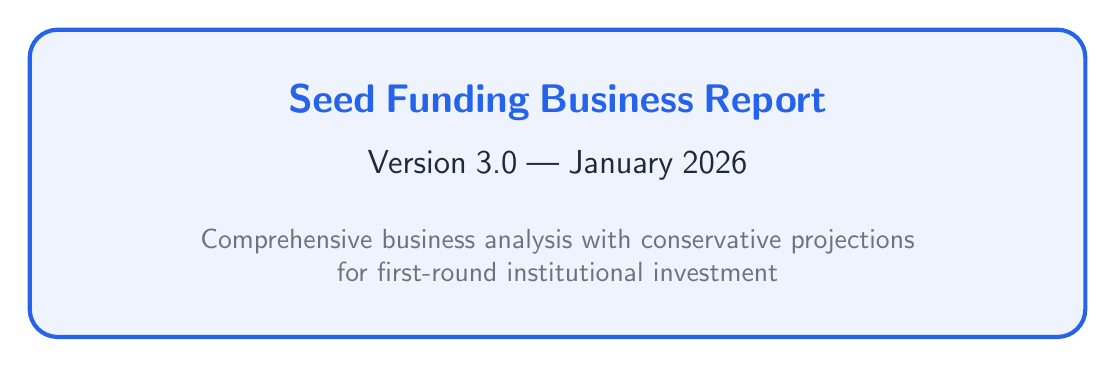
\begin{tikzpicture}
            \node[fill=miloprimary!8, draw=miloprimary, line width=1.5pt, rounded corners=10pt,
                  inner sep=20pt, text width=12cm, align=center] {
                {\Large\textcolor{miloprimary}{\textbf{Seed Funding Business Report}}}\\[10pt]
                {\large\textcolor{darktext}{Version 3.0 | January 2026}}\\[15pt]
                \textcolor{freegray}{Comprehensive business analysis with conservative projections}\\
                \textcolor{freegray}{for first-round institutional investment}
            };
        \end{tikzpicture}

        \vspace{2.5cm}

        % Key metrics preview
        
\begin{tikzpicture}
            \node[fill=successgreen!10, draw=successgreen, line width=1pt, rounded corners=8pt,
                  inner sep=12pt] at (0,0) {
                \textcolor{darkgreen}{\textbf{Year 3 Revenue: \$1.8M}}
            };
            \node[fill=miloprimary!10, draw=miloprimary, line width=1pt, rounded corners=8pt,
                  inner sep=12pt] at (5.5,0) {
                \textcolor{miloprimary}{\textbf{Operating Margin: 45\%}}
            };
            \node[fill=datapurple!10, draw=datapurple, line width=1pt, rounded corners=8pt,
                  inner sep=12pt] at (11,0) {
                \textcolor{datapurple}{\textbf{Break-even: Year 2}}
            };
        \end{tikzpicture}

        \vfill

        {\large\textcolor{miloprimary}{\textbf{DeepmAInd B.V.}}}\\[0.3cm]
        {\textcolor{freegray}{The Netherlands | Confidential}}

    \end{center}
\end{titlepage}

% ============================================================================
% TABLE OF CONTENTS
% ============================================================================
\tableofcontents
\thispagestyle{empty}
\newpage

% ============================================================================
% CHAPTER 1: EXECUTIVE SUMMARY
% ============================================================================
\chapter{Executive Summary}

\section{Investment Opportunity}

\begin{center}
\alertbox{miloprimary}{MILO: Creating a New Category in Consumer Finance}{
MILO creates \textbf{``Wellness-Aware Spending Analytics''}---the intersection of receipt-based spending tracking and health-conscious consumer insights. No competitor currently occupies this unique market position.

\vspace{8pt}
The business model is built on \textbf{three diversified revenue streams}: B2C subscriptions, B2B dataset monetization, and analytics reports. Under conservative assumptions, MILO achieves \textbf{operating profitability in Year 2} with \textbf{45\% operating margins by Year 3}.
}
\end{center}

\vspace{0.5cm}

\begin{center}
    \statbox{dangerred}{Year 1 Loss}{(\$152K)}
    \hspace{0.2cm}
    \statbox{successgreen}{Year 2 Profit}{\$94K}
    \hspace{0.2cm}
    \statbox{darkgreen}{Year 3 Profit}{\$813K}
    \hspace{0.2cm}
    \statbox{miloprimary}{Y3 Margin}{45\%}
\end{center}

\vspace{0.5cm}

\begin{center}
    \revenuestream{appstoreblue}{App Store}{951K}{53\% of Revenue}
    \hspace{0.3cm}
    \revenuestream{datapurple}{Datasets}{637K}{35\% of Revenue}
    \hspace{0.3cm}
    \revenuestream{analyticsteal}{Analytics}{212K}{12\% of Revenue}
\end{center}

\section{Financial Summary}

\begin{center}
\renewcommand{\arraystretch}{1.5}
\begin{tabular}{>{\raggedright\arraybackslash}p{5cm} >{\centering\arraybackslash}p{2.5cm} >{\centering\arraybackslash}p{2.5cm} >{\centering\arraybackslash}p{2.5cm}}
\toprule
\rowcolor{miloprimary!15}
\textbf{Metric} & \textbf{Year 1} & \textbf{Year 2} & \textbf{Year 3} \\
\midrule
\textbf{Total Revenue} & \$144K & \$720K & \$1.8M \\
\rowcolor{lightbg}
\textbf{Total Costs} & \$296K & \$626K & \$987K \\
\textbf{Operating Profit/(Loss)} & (\$152K) & \$94K & \$813K \\
\rowcolor{successgreen!15}
\textbf{Operating Margin} & -106\% & \textbf{13\%} & \textbf{45\%} \\
\midrule
\textbf{Paid Subscribers (EOY)} & 2,000 & 8,000 & 18,000 \\
\rowcolor{lightbg}
\textbf{LTV:CAC Ratio} & 2.1:1 & 3.4:1 & 4.3:1 \\
\bottomrule
\end{tabular}
\end{center}

\section{The Investment Ask}

\begin{center}
\infobox{miloprimary}{
    {\Large\textcolor{miloprimary}{\textbf{Seed Round: \$300K}}}\\[12pt]
    \begin{minipage}[t]{0.48\textwidth}
        \textbf{Use of Funds:}
        \begin{itemize}[leftmargin=1.5em, itemsep=3pt]
            \item Engineering \& Product: 35\%
            \item Sales \& Marketing: 25\%
            \item Legal \& GDPR Compliance: 20\%
            \item B2B Sales Development: 10\%
            \item Operations \& Buffer: 10\%
        \end{itemize}
    \end{minipage}
    \hfill
    \begin{minipage}[t]{0.48\textwidth}
        \textbf{Key Terms:}
        \begin{itemize}[leftmargin=1.5em, itemsep=3pt]
            \item Runway: 18 months to profitability
            \item Break-even: Month 18 (base case)
            \item Year 3 valuation target: \$12-15M
            \item Projected return: 6-8x
        \end{itemize}
    \end{minipage}
}
\end{center}

\section{Why Now?}

\begin{center}
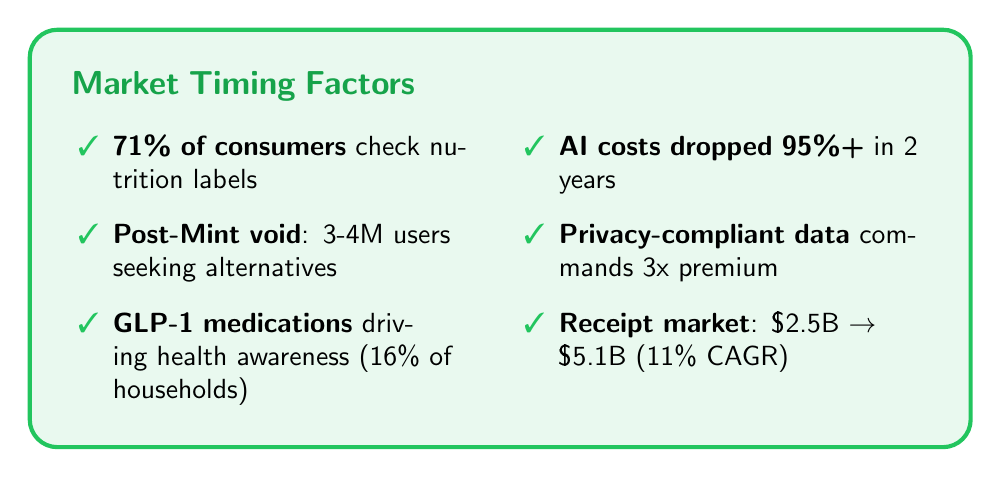
\begin{tikzpicture}
    \node[fill=successgreen!10, draw=successgreen, line width=1.5pt, rounded corners=10pt,
          inner sep=15pt, text width=\textwidth-35pt, align=left] {
        \textcolor{darkgreen}{\textbf{\large Market Timing Factors}}\\[10pt]
        \begin{minipage}[t]{0.48\textwidth}
            \begin{itemize}[leftmargin=1.5em, itemsep=4pt]
                \item[\cmark] \textbf{71\% of consumers} check nutrition labels
                \item[\cmark] \textbf{Post-Mint void}: 3-4M users seeking alternatives
                \item[\cmark] \textbf{GLP-1 medications} driving health awareness (16\% of households)
            \end{itemize}
        \end{minipage}
        \hfill
        \begin{minipage}[t]{0.48\textwidth}
            \begin{itemize}[leftmargin=1.5em, itemsep=4pt]
                \item[\cmark] \textbf{AI costs dropped 95\%+} in 2 years
                \item[\cmark] \textbf{Privacy-compliant data} commands 3x premium
                \item[\cmark] \textbf{Receipt market}: \$2.5B $\rightarrow$ \$5.1B (11\% CAGR)
            \end{itemize}
        \end{minipage}
    };
\end{tikzpicture}
\end{center}

% ============================================================================
% CHAPTER 2: MARKET OPPORTUNITY
% ============================================================================
\chapter{Market Opportunity \& Competitive Landscape}

\section{Market Size}

\begin{center}
\infobox{miloaccent}{
    {\Large\textcolor{miloaccent}{\textbf{Receipt Scanner App Market}}}\\[12pt]
    \begin{minipage}[t]{0.48\textwidth}
        \textbf{Market Size \& Growth}
        \begin{itemize}[leftmargin=1.5em, itemsep=4pt]
            \item \textbf{2024:} \$1.97 billion
            \item \textbf{2033:} \$3.1 billion (projected)
            \item \textbf{CAGR:} 11.2\%
            \item \textbf{Key drivers:} Smartphone adoption, digitalization, AI advancements
        \end{itemize}
    \end{minipage}
    \hfill
    \begin{minipage}[t]{0.48\textwidth}
        \textbf{Adjacent Markets}
        \begin{itemize}[leftmargin=1.5em, itemsep=4pt]
            \item Personal Finance Apps: \$7.2B $\rightarrow$ \$14.4B
            \item Consumer Data Analytics: \$12B $\rightarrow$ \$26.5B
            \item Health/Wellness Apps: Growing 12\%+ annually
        \end{itemize}
    \end{minipage}
}
\end{center}

\section{Competitive Landscape}

\begin{center}
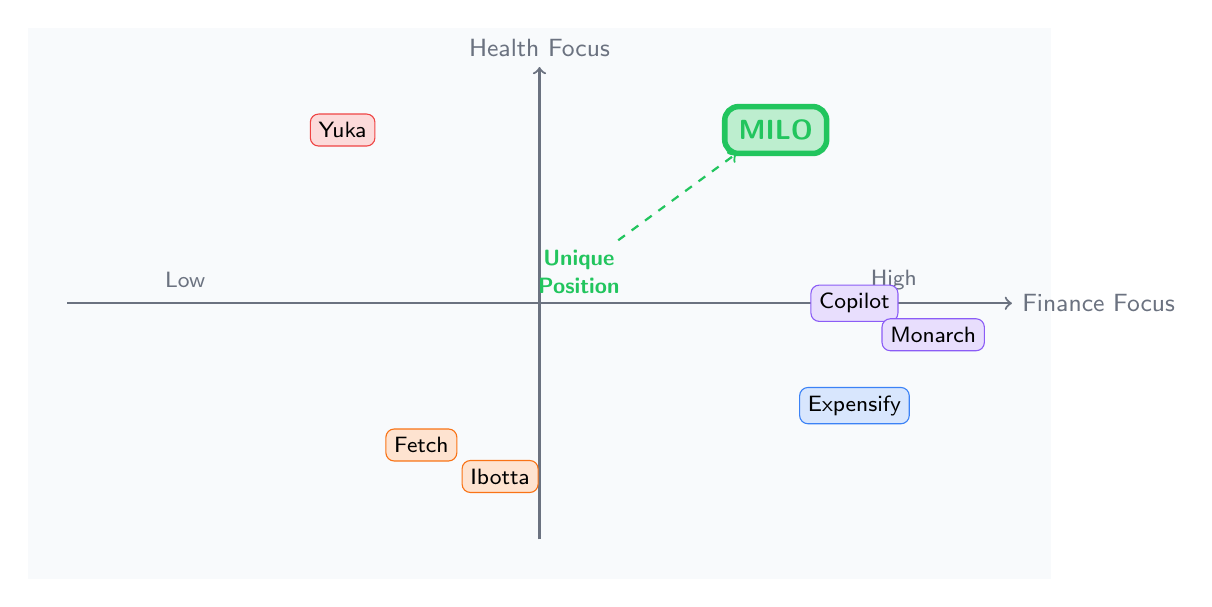
\begin{tikzpicture}
    % Background
    \fill[lightbg] (-6.5,-3.5) rectangle (6.5,3.5);

    % Axes
    \draw[->, thick, freegray] (-6,0) -- (6,0) node[right] {\small\textcolor{freegray}{Finance Focus}};
    \draw[->, thick, freegray] (0,-3) -- (0,3) node[above] {\small\textcolor{freegray}{Health Focus}};

    % Labels
    \node[freegray] at (-4.5,0.3) {\footnotesize Low};
    \node[freegray] at (4.5,0.3) {\footnotesize High};

    % Competitors plotted
    \node[fill=dangerred!20, draw=dangerred, rounded corners=3pt, inner sep=3pt] at (-2.5,2.2) {\footnotesize Yuka};
    \node[fill=warningorange!20, draw=warningorange, rounded corners=3pt, inner sep=3pt] at (-1.5,-1.8) {\footnotesize Fetch};
    \node[fill=warningorange!20, draw=warningorange, rounded corners=3pt, inner sep=3pt] at (-0.5,-2.2) {\footnotesize Ibotta};
    \node[fill=competitorblue!20, draw=competitorblue, rounded corners=3pt, inner sep=3pt] at (4,-1.3) {\footnotesize Expensify};
    \node[fill=datapurple!20, draw=datapurple, rounded corners=3pt, inner sep=3pt] at (4,0) {\footnotesize Copilot};
    \node[fill=datapurple!20, draw=datapurple, rounded corners=3pt, inner sep=3pt] at (5,-0.4) {\footnotesize Monarch};

    % MILO - unique position
    \node[fill=successgreen!30, draw=successgreen, line width=2pt, rounded corners=5pt, inner sep=5pt] at (3,2.2) {\textbf{\textcolor{successgreen}{MILO}}};

    % Arrow pointing to MILO's unique position
    \draw[->, thick, successgreen, dashed] (1,0.8) -- (2.5,1.9);
    \node[successgreen, align=center] at (0.5,0.4) {\footnotesize\textbf{Unique}\\[-2pt]\footnotesize\textbf{Position}};
\end{tikzpicture}
\end{center}

\begin{center}
\alertbox{successgreen}{MILO's Unique Market Position}{
MILO is the \textbf{only consumer app} combining receipt scanning + health scoring + AI-powered spending analytics. This creates a defensive moat at the intersection of personal finance and wellness---a space no competitor currently occupies.
}
\end{center}

\section{Competitive Analysis}

\begin{center}
\renewcommand{\arraystretch}{1.4}
\begin{tabular}{>{\raggedright\arraybackslash}p{3.5cm} >{\centering\arraybackslash}p{2cm} >{\centering\arraybackslash}p{2cm} >{\centering\arraybackslash}p{2cm} >{\centering\arraybackslash}p{2cm}}
\toprule
\rowcolor{miloprimary!15}
\textbf{Feature} & \textbf{MILO} & \textbf{Fetch/Ibotta} & \textbf{Copilot} & \textbf{Expensify} \\
\midrule
Receipt Scanning & \cmark & \cmark & \xmark & \cmark \\
\rowcolor{lightbg}
Health Scores & \cmark & \xmark & \xmark & \xmark \\
Spending Analytics & \cmark & \xmark & \cmark & \cmark \\
\rowcolor{lightbg}
AI Categorization & \cmark & Limited & \cmark & \cmark \\
AI Chat Assistant & \cmark & \xmark & \cmark & \xmark \\
\rowcolor{lightbg}
Item-Level Data & \cmark & \xmark & \xmark & Limited \\
Entry Price & \textcolor{successgreen}{\textbf{\$2/mo}} & Free* & \$13/mo & \$5/user \\
\rowcolor{lightbg}
Target User & Consumers & Deal seekers & Consumers & Businesses \\
\bottomrule
\end{tabular}
\end{center}

{\small *Free but users' data is monetized}

\section{Key Differentiators}

\begin{center}
\infobox{miloprimary}{
    {\Large\textcolor{miloprimary}{\textbf{MILO's Competitive Advantages}}}\\[12pt]
    \begin{minipage}[t]{0.48\textwidth}
        \textbf{\textcolor{successgreen}{1. Unique Market Position}}
        \begin{itemize}[leftmargin=1.2em, itemsep=2pt]
            \item Only app combining receipts + health
            \item Item-level granularity vs transaction-level
            \item Consumer-first (not B2B repackaged)
            \item Privacy-respecting subscription model
        \end{itemize}

        \vspace{8pt}
        \textbf{\textcolor{successgreen}{2. AI-Native Architecture}}
        \begin{itemize}[leftmargin=1.2em, itemsep=2pt]
            \item Built for AI from day one
            \item Intelligent categorization (16 categories)
            \item Health scoring (0--5 scale)
            \item Conversational AI assistant
        \end{itemize}
    \end{minipage}
    \hfill
    \begin{minipage}[t]{0.48\textwidth}
        \textbf{\textcolor{successgreen}{3. Aggressive Pricing}}
        \begin{itemize}[leftmargin=1.2em, itemsep=2pt]
            \item \$2/mo entry---lowest in category
            \item Full features at every tier
            \item Volume-based, not feature-gated
            \item 17\% annual discount
        \end{itemize}

        \vspace{8pt}
        \textbf{\textcolor{successgreen}{4. Three Revenue Streams}}
        \begin{itemize}[leftmargin=1.2em, itemsep=2pt]
            \item B2C subscriptions (stable)
            \item B2B data (high margin)
            \item Analytics reports (scalable)
            \item No single point of failure
        \end{itemize}
    \end{minipage}
}
\end{center}

% ============================================================================
% CHAPTER 3: BUSINESS MODEL
% ============================================================================
\chapter{Business Model \& Pricing Strategy}

\section{Volume-Based Pricing Philosophy}

\begin{center}
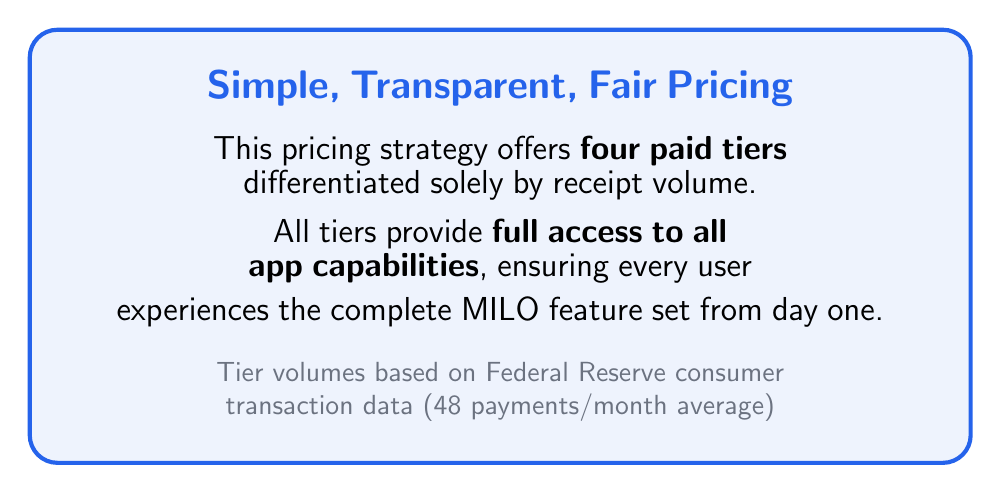
\begin{tikzpicture}
    \node[fill=miloprimary!8, draw=miloprimary, line width=1.5pt, rounded corners=10pt,
          inner sep=15pt, text width=\textwidth-35pt, align=center] {
        {\Large\textcolor{miloprimary}{\textbf{Simple, Transparent, Fair Pricing}}}\\[10pt]
        {\large This pricing strategy offers \textbf{four paid tiers} differentiated solely by receipt volume.}\\[6pt]
        {\large All tiers provide \textbf{full access to all app capabilities}, ensuring every user}\\[4pt]
        {\large experiences the complete MILO feature set from day one.}\\[10pt]
        {\normalsize\textcolor{freegray}{Tier volumes based on Federal Reserve consumer transaction data (48 payments/month average)}}
    };
\end{tikzpicture}
\end{center}

\vspace{0.5cm}

\section{Pricing Tiers}

\begin{center}
    \tierbox{freegray}{FREE TRIAL}{15}{\$0}{14 days}
    \hspace{0.15cm}
    \tierbox{bronzecolor}{BRONZE}{20}{\$2/mo}{\$20/year}
    \hspace{0.15cm}
    \tierbox{silvercolor}{SILVER}{40}{\$4/mo}{\$40/year}
    \hspace{0.15cm}
    \tierbox{goldcolor}{GOLD}{60}{\$6/mo}{\$60/year}
    \hspace{0.15cm}
    \tierbox{platinumcolor}{PLATINUM}{100}{\$10/mo}{\$100/year}
\end{center}

\vspace{0.5cm}

\begin{center}
\renewcommand{\arraystretch}{1.5}
\begin{tabular}{>{\centering\arraybackslash}p{2.2cm} >{\centering\arraybackslash}p{2cm} >{\centering\arraybackslash}p{1.8cm} >{\centering\arraybackslash}p{1.8cm} >{\centering\arraybackslash}p{2cm} >{\centering\arraybackslash}p{3cm}}
\toprule
\rowcolor{miloprimary!15}
\textbf{Tier} & \textbf{Receipts} & \textbf{Monthly} & \textbf{Annual} & \textbf{Per Receipt} & \textbf{Target User} \\
\midrule
\rowcolor{freegray!8}
\textcolor{freegray}{\textbf{Free Trial}} & 15 total & Free & -- & -- & New users \\
\rowcolor{bronzecolor!8}
\textcolor{bronzecolor}{\textbf{Bronze}} & 20/mo & \$2 & \$20 & \$0.10 & Light trackers \\
\rowcolor{silvercolor!8}
\textcolor{silvercolor}{\textbf{Silver}} & 40/mo & \$4 & \$40 & \$0.10 & Average consumers \\
\rowcolor{goldcolor!8}
\textcolor{goldcolor}{\textbf{Gold}} & 60/mo & \$6 & \$60 & \$0.10 & Active trackers \\
\rowcolor{platinumcolor!8}
\textcolor{platinumcolor}{\textbf{Platinum}} & 100/mo & \$10 & \$100 & \$0.10 & Households \\
\bottomrule
\end{tabular}
\end{center}

\vspace{0.3cm}

\begin{center}

\begin{tikzpicture}
    \node[fill=successgreen!10, draw=successgreen, line width=1pt, rounded corners=5pt,
          inner sep=10pt, text width=12cm, align=center] {
        \textcolor{darkgreen}{\textbf{Annual Savings:}} All annual plans offer \textbf{17\% discount} compared to monthly billing
    };
\end{tikzpicture}
\end{center}

\section{Three-Pillar Revenue Model}

\begin{center}
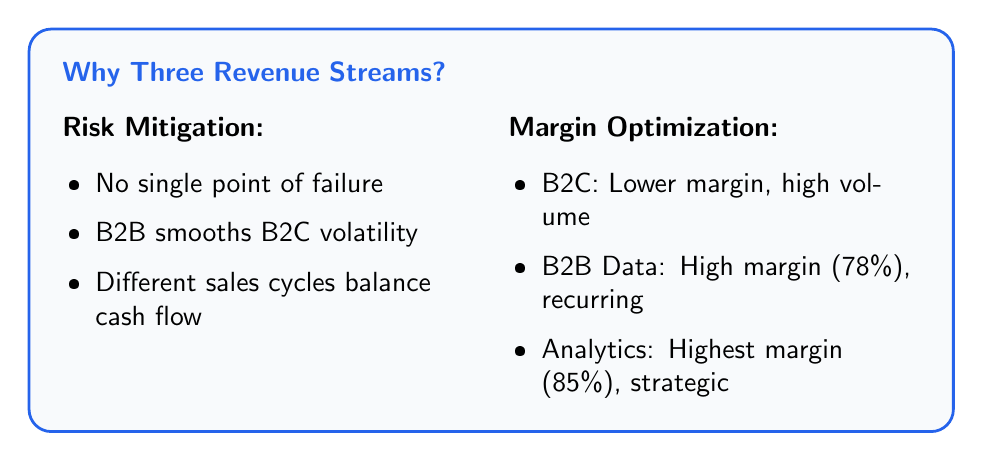
\begin{tikzpicture}
    \node[fill=lightbg, draw=miloprimary, line width=1pt, rounded corners=8pt,
          inner sep=12pt, text width=\textwidth-35pt, align=left] {
        \textcolor{miloprimary}{\textbf{Why Three Revenue Streams?}}\\[8pt]
        \begin{minipage}[t]{0.48\textwidth}
            \textbf{Risk Mitigation:}
            \begin{itemize}[leftmargin=1.2em, itemsep=2pt]
                \item No single point of failure
                \item B2B smooths B2C volatility
                \item Different sales cycles balance cash flow
            \end{itemize}
        \end{minipage}
        \hfill
        \begin{minipage}[t]{0.48\textwidth}
            \textbf{Margin Optimization:}
            \begin{itemize}[leftmargin=1.2em, itemsep=2pt]
                \item B2C: Lower margin, high volume
                \item B2B Data: High margin (78\%), recurring
                \item Analytics: Highest margin (85\%), strategic
            \end{itemize}
        \end{minipage}
    };
\end{tikzpicture}
\end{center}

\vspace{0.3cm}

\begin{center}
\renewcommand{\arraystretch}{1.5}
\begin{tabular}{>{\raggedright\arraybackslash}p{4cm} >{\centering\arraybackslash}p{2cm} >{\centering\arraybackslash}p{2cm} >{\centering\arraybackslash}p{2cm} >{\centering\arraybackslash}p{1.5cm} >{\centering\arraybackslash}p{1.5cm}}
\toprule
\rowcolor{miloprimary!15}
\textbf{Revenue Stream} & \textbf{Year 1} & \textbf{Year 2} & \textbf{Year 3} & \textbf{Y3 \%} & \textbf{Margin} \\
\midrule
\rowcolor{appstoreblue!8}
\textcolor{appstoreblue}{\textbf{App Store (B2C)}} & \$105K & \$423K & \$951K & 53\% & 19\% \\
\rowcolor{datapurple!8}
\textcolor{datapurple}{\textbf{Datasets (B2B)}} & \$28K & \$225K & \$637K & 35\% & 78\% \\
\rowcolor{analyticsteal!8}
\textcolor{analyticsteal}{\textbf{Analytics Reports}} & \$11K & \$72K & \$212K & 12\% & 85\% \\
\midrule
\rowcolor{successgreen!10}
\textbf{Total Revenue} & \textbf{\$144K} & \textbf{\$720K} & \textbf{\$1,800K} & \textbf{100\%} & -- \\
\bottomrule
\end{tabular}
\end{center}

\section{B2B Data Monetization}

\begin{center}
\infobox{datapurple}{
    {\Large\textcolor{datapurple}{\textbf{Premium Consumer Purchase Intelligence}}}\\[10pt]
    MILO's data is differentiated by \textbf{item-level granularity} (10-50 data points per receipt vs. 1-3 for competitors) and \textbf{proprietary health scoring}. All data is explicitly consented, GDPR-compliant, and commands premium pricing.\\[10pt]
    \begin{minipage}[t]{0.48\textwidth}
        \textbf{Data Elements:}
        \begin{itemize}[leftmargin=1.2em, itemsep=2pt]
            \item SKU-level product data
            \item Health scores (0-5 scale)
            \item Shopping frequency patterns
            \item Store/brand preferences
        \end{itemize}
    \end{minipage}
    \hfill
    \begin{minipage}[t]{0.48\textwidth}
        \textbf{Target Buyers:}
        \begin{itemize}[leftmargin=1.2em, itemsep=2pt]
            \item CPG brands (Nestl\'{e}, Unilever)
            \item Retailers (Kroger, Target)
            \item Health/wellness brands
            \item Market research firms
        \end{itemize}
    \end{minipage}
}
\end{center}

% ============================================================================
% CHAPTER 4: FINANCIAL PROJECTIONS
% ============================================================================
\chapter{Financial Projections}

\section{Profit \& Loss Statement}

\begin{center}
\renewcommand{\arraystretch}{1.4}
\begin{tabular}{>{\raggedright\arraybackslash}p{5cm} >{\centering\arraybackslash}p{2.5cm} >{\centering\arraybackslash}p{2.5cm} >{\centering\arraybackslash}p{2.5cm}}
\toprule
\rowcolor{miloprimary!15}
\textbf{Line Item} & \textbf{Year 1} & \textbf{Year 2} & \textbf{Year 3} \\
\midrule
\multicolumn{4}{l}{\textbf{\textcolor{miloprimary}{REVENUE}}} \\
\rowcolor{appstoreblue!5}
\quad App Store (B2C) & \$105K & \$423K & \$951K \\
\rowcolor{datapurple!5}
\quad Dataset Monetization (B2B) & \$28K & \$225K & \$637K \\
\rowcolor{analyticsteal!5}
\quad Analytics Reports & \$11K & \$72K & \$212K \\
\rowcolor{successgreen!10}
\textbf{Total Revenue} & \textbf{\$144K} & \textbf{\$720K} & \textbf{\$1,800K} \\
\midrule
\multicolumn{4}{l}{\textbf{\textcolor{miloprimary}{COST OF REVENUE (Variable)}}} \\
\rowcolor{lightbg}
\quad Veryfi OCR Processing & \$26K & \$83K & \$179K \\
\quad Gemini API & \$1K & \$3K & \$6K \\
\rowcolor{lightbg}
\quad Firebase/Storage & \$1K & \$4K & \$8K \\
\quad Payment Processing (Apple 15\%) & \$8K & \$26K & \$39K \\
\rowcolor{warningorange!8}
\textbf{Total Variable Costs} & \textbf{\$36K} & \textbf{\$116K} & \textbf{\$232K} \\
\midrule
\rowcolor{successgreen!8}
\textbf{GROSS PROFIT} & \textbf{\$108K} & \textbf{\$604K} & \textbf{\$1,568K} \\
\rowcolor{successgreen!15}
\textbf{Gross Margin} & \textbf{75\%} & \textbf{84\%} & \textbf{87\%} \\
\midrule
\multicolumn{4}{l}{\textbf{\textcolor{miloprimary}{OPERATING EXPENSES (Fixed)}}} \\
\rowcolor{lightbg}
\quad Engineering \& Product & \$100K & \$180K & \$300K \\
\quad Sales \& Marketing & \$75K & \$150K & \$200K \\
\rowcolor{lightbg}
\quad B2B Sales Team & \$25K & \$80K & \$120K \\
\quad Legal \& Compliance (GDPR) & \$40K & \$60K & \$75K \\
\rowcolor{lightbg}
\quad Customer Support & \$10K & \$25K & \$40K \\
\quad Infrastructure (non-API) & \$10K & \$15K & \$20K \\
\rowcolor{miloprimary!8}
\textbf{Total Operating Expenses} & \textbf{\$260K} & \textbf{\$510K} & \textbf{\$755K} \\
\midrule
\rowcolor{dangerred!10}
\textbf{OPERATING PROFIT/(LOSS)} & \textbf{(\$152K)} & \textbf{\$94K} & \textbf{\$813K} \\
\rowcolor{miloprimary!15}
\textbf{Operating Margin} & \textbf{-106\%} & \textbf{13\%} & \textbf{45\%} \\
\bottomrule
\end{tabular}
\end{center}

\section{User Growth Projections}

\begin{center}
\renewcommand{\arraystretch}{1.4}
\begin{tabular}{>{\raggedright\arraybackslash}p{4.5cm} >{\centering\arraybackslash}p{3cm} >{\centering\arraybackslash}p{3cm} >{\centering\arraybackslash}p{3cm}}
\toprule
\rowcolor{miloprimary!15}
\textbf{Metric} & \textbf{Year 1} & \textbf{Year 2} & \textbf{Year 3} \\
\midrule
Total App Downloads & 25,000 & 80,000 & 150,000 \\
\rowcolor{lightbg}
Free Trial Users & 15,000 & 48,000 & 90,000 \\
Trial-to-Paid Conversion & 13\% & 17\% & 20\% \\
\rowcolor{lightbg}
\textbf{Paid Subscribers (EOY)} & \textbf{2,000} & \textbf{8,000} & \textbf{18,000} \\
Monthly Churn Rate & 5\% & 4\% & 3.5\% \\
\rowcolor{lightbg}
Net Subscriber Retention & 95\% & 96\% & 96.5\% \\
\bottomrule
\end{tabular}
\end{center}

\begin{center}
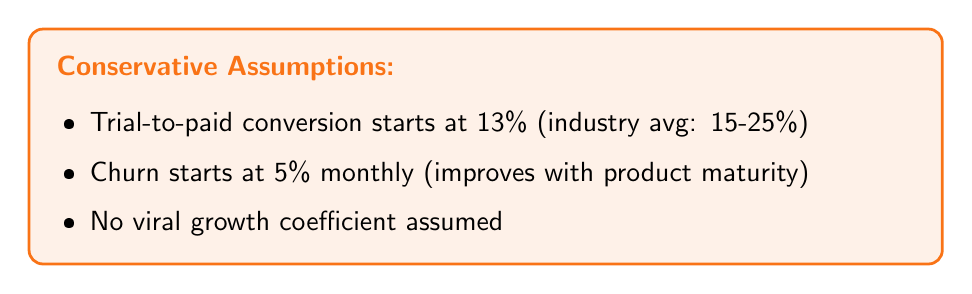
\begin{tikzpicture}
    \node[fill=warningorange!10, draw=warningorange, line width=1pt, rounded corners=5pt,
          inner sep=10pt, text width=\textwidth-35pt, align=left] {
        \textcolor{warningorange}{\textbf{Conservative Assumptions:}}
        \begin{itemize}[leftmargin=1.2em, itemsep=2pt]
            \item Trial-to-paid conversion starts at 13\% (industry avg: 15-25\%)
            \item Churn starts at 5\% monthly (improves with product maturity)
            \item No viral growth coefficient assumed
        \end{itemize}
    };
\end{tikzpicture}
\end{center}

\section{Tier Distribution \& Revenue}

\begin{center}
\renewcommand{\arraystretch}{1.4}
\begin{tabular}{>{\raggedright\arraybackslash}p{2.5cm} >{\centering\arraybackslash}p{1.3cm} >{\centering\arraybackslash}p{1.5cm} >{\centering\arraybackslash}p{2cm} >{\centering\arraybackslash}p{2cm} >{\centering\arraybackslash}p{2cm}}
\toprule
\rowcolor{miloprimary!15}
\textbf{Tier} & \textbf{Price} & \textbf{Mix} & \textbf{Y1 Rev} & \textbf{Y2 Rev} & \textbf{Y3 Rev} \\
\midrule
\rowcolor{bronzecolor!8}
\textcolor{bronzecolor}{\textbf{Bronze}} & \$2/mo & 30\% & \$14K & \$58K & \$130K \\
\rowcolor{silvercolor!8}
\textcolor{silvercolor}{\textbf{Silver}} & \$4/mo & 40\% & \$38K & \$154K & \$346K \\
\rowcolor{goldcolor!8}
\textcolor{goldcolor}{\textbf{Gold}} & \$6/mo & 20\% & \$29K & \$115K & \$259K \\
\rowcolor{platinumcolor!8}
\textcolor{platinumcolor}{\textbf{Platinum}} & \$10/mo & 10\% & \$24K & \$96K & \$216K \\
\midrule
\rowcolor{lightbg}
\textbf{Gross App Revenue} & -- & 100\% & \$105K & \$423K & \$951K \\
\rowcolor{dangerred!8}
\textit{Less: Apple (15\%)} & -- & -- & (\$16K) & (\$63K) & (\$143K) \\
\rowcolor{successgreen!10}
\textbf{Net App Store Rev} & -- & -- & \textbf{\$89K} & \textbf{\$360K} & \textbf{\$808K} \\
\bottomrule
\end{tabular}
\end{center}

\section{Cash Flow Analysis}

\begin{center}
\renewcommand{\arraystretch}{1.4}
\begin{tabular}{>{\raggedright\arraybackslash}p{5cm} >{\centering\arraybackslash}p{3cm} >{\centering\arraybackslash}p{3cm} >{\centering\arraybackslash}p{3cm}}
\toprule
\rowcolor{miloprimary!15}
\textbf{Cash Flow Item} & \textbf{Year 1} & \textbf{Year 2} & \textbf{Year 3} \\
\midrule
Operating Cash Flow & (\$152K) & \$94K & \$813K \\
\rowcolor{lightbg}
Beginning Cash (with \$300K funding) & \$300K & \$148K & \$242K \\
\textbf{Ending Cash Position} & \textbf{\$148K} & \textbf{\$242K} & \textbf{\$1,055K} \\
\rowcolor{successgreen!10}
\textbf{Months Runway} & 9 months & 5 months & 17 months \\
\bottomrule
\end{tabular}
\end{center}

\begin{center}
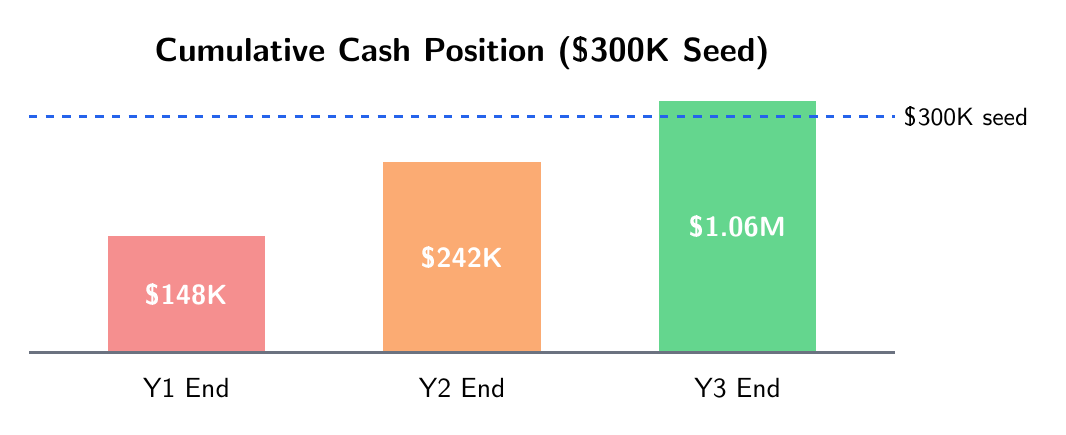
\begin{tikzpicture}
    % Title
    \node[align=center] at (0,3.8) {\textbf{\large Cumulative Cash Position (\$300K Seed)}};

    % Bars
    \fill[dangerred!60] (-4.5,0) rectangle (-2.5,1.48);
    \node at (-3.5,0.74) {\textcolor{white}{\textbf{\$148K}}};
    \node[below] at (-3.5,-0.2) {Y1 End};

    \fill[warningorange!60] (-1,0) rectangle (1,2.42);
    \node at (0,1.21) {\textcolor{white}{\textbf{\$242K}}};
    \node[below] at (0,-0.2) {Y2 End};

    \fill[successgreen!70] (2.5,0) rectangle (4.5,3.2);
    \node at (3.5,1.6) {\textcolor{white}{\textbf{\$1.06M}}};
    \node[below] at (3.5,-0.2) {Y3 End};

    % Baseline
    \draw[line width=1pt, freegray] (-5.5,0) -- (5.5,0);

    % Reference line for seed
    \draw[dashed, line width=1pt, miloprimary] (-5.5,3) -- (5.5,3);
    \node[right] at (5.5,3) {\small \$300K seed};
\end{tikzpicture}
\end{center}

% ============================================================================
% CHAPTER 5: COST STRUCTURE
% ============================================================================
\chapter{Cost Structure \& Unit Economics}

\section{Variable Costs by Tier}

\begin{center}
\renewcommand{\arraystretch}{1.5}
\begin{tabular}{>{\raggedright\arraybackslash}p{3.5cm} >{\centering\arraybackslash}p{1.8cm} >{\centering\arraybackslash}p{1.8cm} >{\centering\arraybackslash}p{1.8cm} >{\centering\arraybackslash}p{1.8cm} >{\centering\arraybackslash}p{1.8cm}}
\toprule
\rowcolor{miloprimary!15}
\textbf{Component} & \textbf{Trial} & \textbf{Bronze} & \textbf{Silver} & \textbf{Gold} & \textbf{Platinum} \\
\midrule
\textbf{Receipt Limit} & 15 & 20 & 40 & 60 & 100 \\
\rowcolor{lightbg}
\textbf{Veryfi OCR (\$0.08)} & \$1.20 & \$1.60 & \$3.20 & \$4.80 & \$8.00 \\
\textbf{Gemini API} & \$0.01 & \$0.02 & \$0.03 & \$0.05 & \$0.08 \\
\rowcolor{lightbg}
\textbf{Firebase Storage} & \$0.01 & \$0.01 & \$0.01 & \$0.02 & \$0.02 \\
\midrule
\rowcolor{warningorange!10}
\textbf{Total Variable Cost} & \textbf{\$1.22} & \textbf{\$1.63} & \textbf{\$3.24} & \textbf{\$4.87} & \textbf{\$8.10} \\
\bottomrule
\end{tabular}
\end{center}

\section{Gross Margin by Tier}

\begin{center}
\renewcommand{\arraystretch}{1.5}
\begin{tabular}{>{\raggedright\arraybackslash}p{2.5cm} >{\centering\arraybackslash}p{1.5cm} >{\centering\arraybackslash}p{2cm} >{\centering\arraybackslash}p{2cm} >{\centering\arraybackslash}p{2cm} >{\centering\arraybackslash}p{2.5cm}}
\toprule
\rowcolor{miloprimary!15}
\textbf{Tier} & \textbf{Price} & \textbf{Variable Cost} & \textbf{Gross Profit} & \textbf{Gross Margin} & \textbf{Status} \\
\midrule
\rowcolor{freegray!8}
\textcolor{freegray}{\textbf{Free Trial}} & \$0.00 & \$1.22 & -\$1.22 & -100\% & \cellcolor{freegray!15}\textcolor{freegray}{CAC Investment} \\
\rowcolor{bronzecolor!10}
\textcolor{bronzecolor}{\textbf{Bronze}} & \$2.00 & \$1.63 & \$0.37 & \textbf{18.5\%} & \cellcolor{successgreen!20}\textcolor{darkgreen}{\textbf{Healthy}} \\
\rowcolor{silvercolor!10}
\textcolor{silvercolor}{\textbf{Silver}} & \$4.00 & \$3.24 & \$0.76 & \textbf{19.0\%} & \cellcolor{successgreen!20}\textcolor{darkgreen}{\textbf{Healthy}} \\
\rowcolor{goldcolor!10}
\textcolor{goldcolor}{\textbf{Gold}} & \$6.00 & \$4.87 & \$1.13 & \textbf{18.8\%} & \cellcolor{successgreen!20}\textcolor{darkgreen}{\textbf{Healthy}} \\
\rowcolor{platinumcolor!10}
\textcolor{platinumcolor}{\textbf{Platinum}} & \$10.00 & \$8.10 & \$1.90 & \textbf{19.0\%} & \cellcolor{successgreen!20}\textcolor{darkgreen}{\textbf{Healthy}} \\
\bottomrule
\end{tabular}
\end{center}

\begin{center}
\alertbox{successgreen}{All Paid Tiers Achieve Positive Gross Margins}{
\begin{itemize}[leftmargin=1.5em, itemsep=3pt]
    \item \textbf{Consistent margins:} All tiers maintain 18.5--19\% gross margins
    \item \textbf{Scalable pricing:} Higher tiers provide more value with maintained profitability
    \item \textbf{Blended average:} 19\% gross margin across all paid tiers (weighted by expected mix)
\end{itemize}
}
\end{center}

\section{Customer Lifetime Value (LTV)}

\begin{center}
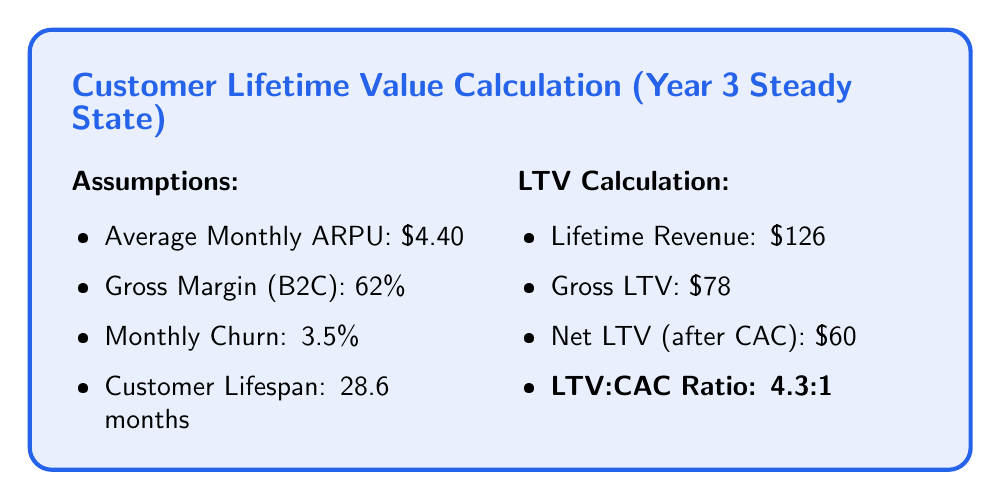
\begin{tikzpicture}
    \node[fill=miloprimary!10, draw=miloprimary, line width=1.5pt, rounded corners=8pt,
          inner sep=15pt, text width=\textwidth-35pt, align=left] {
        \textcolor{miloprimary}{\textbf{\large Customer Lifetime Value Calculation (Year 3 Steady State)}}\\[10pt]
        \begin{minipage}[t]{0.48\textwidth}
            \textbf{Assumptions:}
            \begin{itemize}[leftmargin=1.2em, itemsep=2pt]
                \item Average Monthly ARPU: \$4.40
                \item Gross Margin (B2C): 62\%
                \item Monthly Churn: 3.5\%
                \item Customer Lifespan: 28.6 months
            \end{itemize}
        \end{minipage}
        \hfill
        \begin{minipage}[t]{0.48\textwidth}
            \textbf{LTV Calculation:}
            \begin{itemize}[leftmargin=1.2em, itemsep=2pt]
                \item Lifetime Revenue: \$126
                \item Gross LTV: \$78
                \item Net LTV (after CAC): \$60
                \item \textbf{LTV:CAC Ratio: 4.3:1}
            \end{itemize}
        \end{minipage}
    };
\end{tikzpicture}
\end{center}

\vspace{0.5cm}

\begin{center}
\renewcommand{\arraystretch}{1.4}
\begin{tabular}{>{\raggedright\arraybackslash}p{2.5cm} >{\centering\arraybackslash}p{1.8cm} >{\centering\arraybackslash}p{2.2cm} >{\centering\arraybackslash}p{2.2cm} >{\centering\arraybackslash}p{1.8cm} >{\centering\arraybackslash}p{1.8cm}}
\toprule
\rowcolor{miloprimary!15}
\textbf{Tier} & \textbf{Price} & \textbf{Lifetime Rev} & \textbf{Gross LTV} & \textbf{CAC} & \textbf{LTV:CAC} \\
\midrule
\rowcolor{bronzecolor!8}
\textcolor{bronzecolor}{\textbf{Bronze}} & \$2/mo & \$57 & \$35 & \$18 & 1.9:1 \\
\rowcolor{silvercolor!8}
\textcolor{silvercolor}{\textbf{Silver}} & \$4/mo & \$114 & \$71 & \$18 & 3.9:1 \\
\rowcolor{goldcolor!8}
\textcolor{goldcolor}{\textbf{Gold}} & \$6/mo & \$172 & \$107 & \$18 & 5.9:1 \\
\rowcolor{platinumcolor!8}
\textcolor{platinumcolor}{\textbf{Platinum}} & \$10/mo & \$286 & \$177 & \$18 & 9.8:1 \\
\midrule
\rowcolor{successgreen!10}
\textbf{Blended Average} & \$4.40/mo & \$126 & \$78 & \$18 & \textbf{4.3:1} \\
\bottomrule
\end{tabular}
\end{center}

\begin{center}
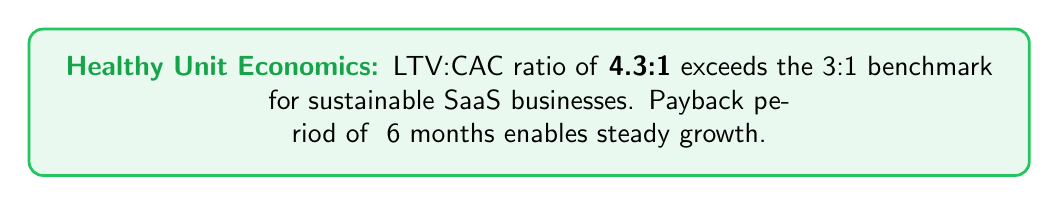
\begin{tikzpicture}
    \node[fill=successgreen!10, draw=successgreen, line width=1pt, rounded corners=5pt,
          inner sep=10pt, text width=12cm, align=center] {
        \textcolor{darkgreen}{\textbf{Healthy Unit Economics:}} LTV:CAC ratio of \textbf{4.3:1} exceeds the 3:1 benchmark\\for sustainable SaaS businesses. Payback period of ~6 months enables steady growth.
    };
\end{tikzpicture}
\end{center}

\section{Fixed Cost Structure}

\begin{center}
\renewcommand{\arraystretch}{1.4}
\begin{tabular}{>{\raggedright\arraybackslash}p{4.5cm} >{\centering\arraybackslash}p{2.5cm} >{\centering\arraybackslash}p{2.5cm} >{\centering\arraybackslash}p{2.5cm}}
\toprule
\rowcolor{miloprimary!15}
\textbf{Category} & \textbf{Year 1} & \textbf{Year 2} & \textbf{Year 3} \\
\midrule
\textbf{Engineering \& Product} & \$100K & \$180K & \$300K \\
\rowcolor{lightbg}
\textbf{Sales \& Marketing} & \$75K & \$150K & \$200K \\
\textbf{B2B Sales Team} & \$25K & \$80K & \$120K \\
\rowcolor{lightbg}
\textbf{Legal \& Compliance (GDPR)} & \$40K & \$60K & \$75K \\
\textbf{Customer Support} & \$10K & \$25K & \$40K \\
\rowcolor{lightbg}
\textbf{Infrastructure (non-API)} & \$10K & \$15K & \$20K \\
\midrule
\rowcolor{miloprimary!15}
\textbf{Total Fixed Costs} & \textbf{\$260K} & \textbf{\$510K} & \textbf{\$755K} \\
\textbf{Fixed Cost per User} & \$130 & \$64 & \$42 \\
\bottomrule
\end{tabular}
\end{center}

\begin{center}
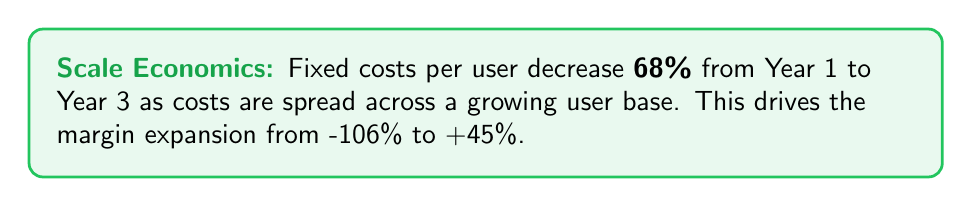
\begin{tikzpicture}
    \node[fill=successgreen!10, draw=successgreen, line width=1pt, rounded corners=5pt,
          inner sep=10pt, text width=\textwidth-35pt, align=left] {
        \textcolor{darkgreen}{\textbf{Scale Economics:}} Fixed costs per user decrease \textbf{68\%} from Year 1 to Year 3 as costs are spread across a growing user base. This drives the margin expansion from -106\% to +45\%.
    };
\end{tikzpicture}
\end{center}

% ============================================================================
% CHAPTER 6: RISK ANALYSIS
% ============================================================================
\chapter{Risk Analysis \& Mitigation}

\section{Sensitivity Analysis}

\begin{center}
\renewcommand{\arraystretch}{1.4}
\begin{tabular}{>{\raggedright\arraybackslash}p{4cm} >{\centering\arraybackslash}p{2cm} >{\centering\arraybackslash}p{2cm} >{\centering\arraybackslash}p{2cm} >{\centering\arraybackslash}p{2cm}}
\toprule
\rowcolor{miloprimary!15}
\textbf{Variable} & \textbf{-20\%} & \textbf{Base Case} & \textbf{+20\%} & \textbf{Impact} \\
\midrule
\rowcolor{dangerred!10}
Trial Conversion Rate & \$493K & \$813K & \$1,133K & \cellcolor{dangerred!20}\textbf{HIGH} \\
\rowcolor{dangerred!10}
Data Consent Rate & \$685K & \$813K & \$941K & \cellcolor{dangerred!20}\textbf{HIGH} \\
\rowcolor{warningorange!10}
User Churn Rate & \$973K & \$813K & \$653K & \cellcolor{warningorange!20}MEDIUM \\
\rowcolor{warningorange!10}
Veryfi OCR Costs & \$849K & \$813K & \$777K & \cellcolor{warningorange!20}MEDIUM \\
\rowcolor{successgreen!10}
Engineering Costs & \$873K & \$813K & \$753K & \cellcolor{successgreen!20}LOW \\
\bottomrule
\end{tabular}
\end{center}

\section{Scenario Analysis}

\begin{center}
\renewcommand{\arraystretch}{1.4}
\begin{tabular}{>{\raggedright\arraybackslash}p{3.5cm} >{\centering\arraybackslash}p{2cm} >{\centering\arraybackslash}p{2cm} >{\centering\arraybackslash}p{2cm} >{\centering\arraybackslash}p{2cm} >{\centering\arraybackslash}p{1.5cm}}
\toprule
\rowcolor{miloprimary!15}
\textbf{Scenario} & \textbf{Year 1} & \textbf{Year 2} & \textbf{Year 3} & \textbf{3-Yr Total} & \textbf{Prob.} \\
\midrule
\rowcolor{dangerred!10}
\textbf{Bear Case} & (\$190K) & (\$50K) & \$350K & \$110K & 20\% \\
\rowcolor{lightbg}
\textbf{Base Case} & (\$152K) & \$94K & \$813K & \$755K & 60\% \\
\rowcolor{successgreen!10}
\textbf{Bull Case} & (\$100K) & \$250K & \$1,300K & \$1,450K & 20\% \\
\midrule
\rowcolor{miloprimary!10}
\textbf{Expected Value} & (\$146K) & \$87K & \$761K & \textbf{\$702K} & -- \\
\bottomrule
\end{tabular}
\end{center}

\section{Key Risks \& Mitigations}

\begin{center}
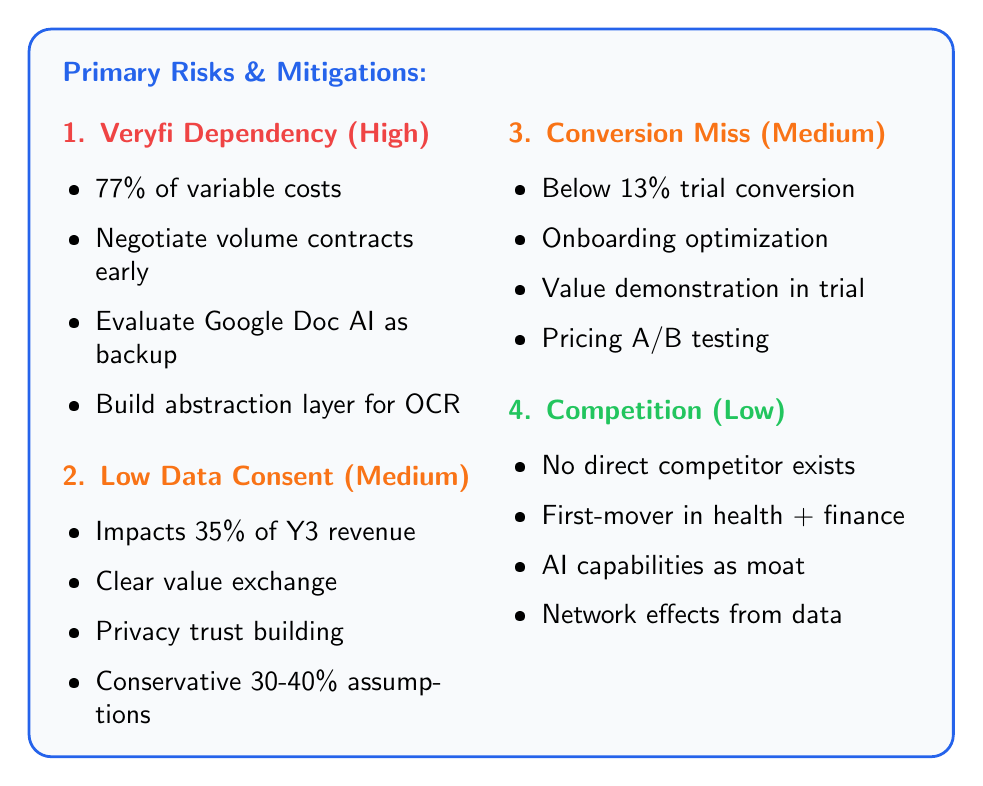
\begin{tikzpicture}
    \node[fill=lightbg, draw=miloprimary, line width=1pt, rounded corners=8pt,
          inner sep=12pt, text width=\textwidth-35pt, align=left] {
        \textcolor{miloprimary}{\textbf{Primary Risks \& Mitigations:}}\\[10pt]
        \begin{minipage}[t]{0.48\textwidth}
            \textcolor{dangerred}{\textbf{1. Veryfi Dependency (High)}}
            \begin{itemize}[leftmargin=1.2em, itemsep=2pt]
                \item 77\% of variable costs
                \item Negotiate volume contracts early
                \item Evaluate Google Doc AI as backup
                \item Build abstraction layer for OCR
            \end{itemize}
            \vspace{6pt}
            \textcolor{warningorange}{\textbf{2. Low Data Consent (Medium)}}
            \begin{itemize}[leftmargin=1.2em, itemsep=2pt]
                \item Impacts 35\% of Y3 revenue
                \item Clear value exchange
                \item Privacy trust building
                \item Conservative 30-40\% assumptions
            \end{itemize}
        \end{minipage}
        \hfill
        \begin{minipage}[t]{0.48\textwidth}
            \textcolor{warningorange}{\textbf{3. Conversion Miss (Medium)}}
            \begin{itemize}[leftmargin=1.2em, itemsep=2pt]
                \item Below 13\% trial conversion
                \item Onboarding optimization
                \item Value demonstration in trial
                \item Pricing A/B testing
            \end{itemize}
            \vspace{6pt}
            \textcolor{successgreen}{\textbf{4. Competition (Low)}}
            \begin{itemize}[leftmargin=1.2em, itemsep=2pt]
                \item No direct competitor exists
                \item First-mover in health + finance
                \item AI capabilities as moat
                \item Network effects from data
            \end{itemize}
        \end{minipage}
    };
\end{tikzpicture}
\end{center}

\section{Revenue Risk Matrix}

\begin{center}
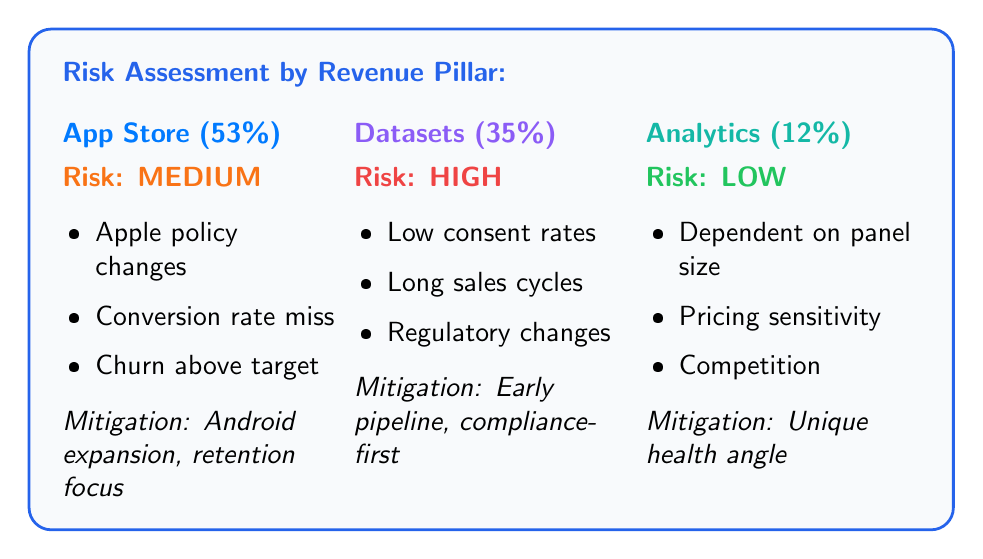
\begin{tikzpicture}
    \node[fill=lightbg, draw=miloprimary, line width=1pt, rounded corners=8pt,
          inner sep=12pt, text width=\textwidth-35pt, align=left] {
        \textcolor{miloprimary}{\textbf{Risk Assessment by Revenue Pillar:}}\\[10pt]
        \begin{minipage}[t]{0.32\textwidth}
            \textcolor{appstoreblue}{\textbf{App Store (53\%)}}\\[4pt]
            \textcolor{warningorange}{\textbf{Risk: MEDIUM}}
            \begin{itemize}[leftmargin=1.2em, itemsep=2pt]
                \item Apple policy changes
                \item Conversion rate miss
                \item Churn above target
            \end{itemize}
            \textit{Mitigation: Android expansion, retention focus}
        \end{minipage}
        \hfill
        \begin{minipage}[t]{0.32\textwidth}
            \textcolor{datapurple}{\textbf{Datasets (35\%)}}\\[4pt]
            \textcolor{dangerred}{\textbf{Risk: HIGH}}
            \begin{itemize}[leftmargin=1.2em, itemsep=2pt]
                \item Low consent rates
                \item Long sales cycles
                \item Regulatory changes
            \end{itemize}
            \textit{Mitigation: Early pipeline, compliance-first}
        \end{minipage}
        \hfill
        \begin{minipage}[t]{0.32\textwidth}
            \textcolor{analyticsteal}{\textbf{Analytics (12\%)}}\\[4pt]
            \textcolor{successgreen}{\textbf{Risk: LOW}}
            \begin{itemize}[leftmargin=1.2em, itemsep=2pt]
                \item Dependent on panel size
                \item Pricing sensitivity
                \item Competition
            \end{itemize}
            \textit{Mitigation: Unique health angle}
        \end{minipage}
    };
\end{tikzpicture}
\end{center}

\begin{center}
\alertbox{infoblue}{Diversification Benefit}{
The three-pillar model provides natural hedging:
\begin{itemize}[leftmargin=1.5em, itemsep=3pt]
    \item If B2C underperforms, B2B provides stability (longer contracts, predictable revenue)
    \item If B2B sales slow, B2C subscription base continues growing
    \item Analytics revenue requires minimal incremental cost once panel is established
    \item No single revenue stream exceeds 55\% of total by Year 3
\end{itemize}
}
\end{center}

% ============================================================================
% CHAPTER 7: CONCLUSION & INVESTMENT THESIS
% ============================================================================
\chapter{Conclusion \& Investment Thesis}

\section{Key Strengths}

\begin{center}
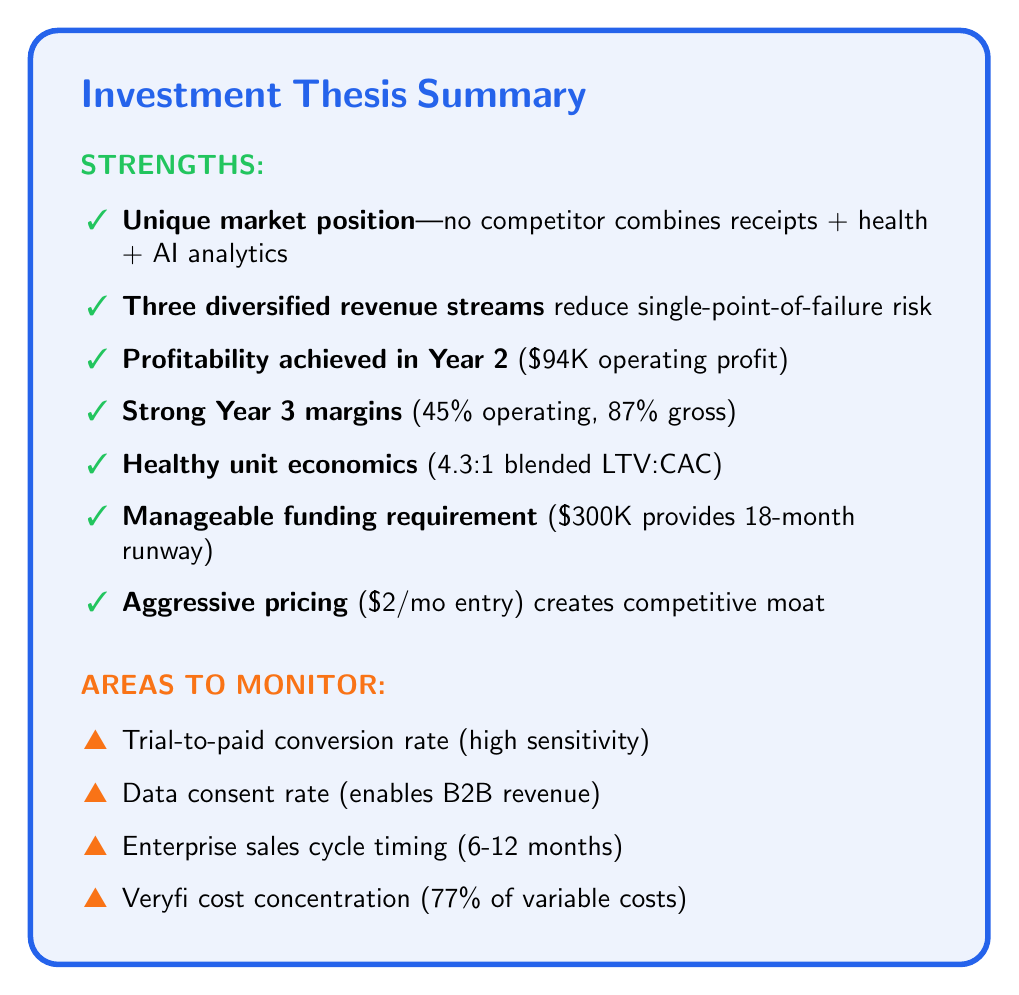
\begin{tikzpicture}
    \node[fill=miloprimary!8, draw=miloprimary, line width=2pt, rounded corners=10pt,
          inner sep=18pt, text width=\textwidth-35pt, align=left] {
        {\Large\textcolor{miloprimary}{\textbf{Investment Thesis Summary}}}\\[12pt]

        \textcolor{successgreen}{\textbf{STRENGTHS:}}
        \begin{itemize}[leftmargin=1.5em, itemsep=3pt]
            \item[\cmark] \textbf{Unique market position}---no competitor combines receipts + health + AI analytics
            \item[\cmark] \textbf{Three diversified revenue streams} reduce single-point-of-failure risk
            \item[\cmark] \textbf{Profitability achieved in Year 2} (\$94K operating profit)
            \item[\cmark] \textbf{Strong Year 3 margins} (45\% operating, 87\% gross)
            \item[\cmark] \textbf{Healthy unit economics} (4.3:1 blended LTV:CAC)
            \item[\cmark] \textbf{Manageable funding requirement} (\$300K provides 18-month runway)
            \item[\cmark] \textbf{Aggressive pricing} (\$2/mo entry) creates competitive moat
        \end{itemize}

        \vspace{10pt}
        \textcolor{warningorange}{\textbf{AREAS TO MONITOR:}}
        \begin{itemize}[leftmargin=1.5em, itemsep=3pt]
            \item[\wmark] Trial-to-paid conversion rate (high sensitivity)
            \item[\wmark] Data consent rate (enables B2B revenue)
            \item[\wmark] Enterprise sales cycle timing (6-12 months)
            \item[\wmark] Veryfi cost concentration (77\% of variable costs)
        \end{itemize}
    };
\end{tikzpicture}
\end{center}

\section{Key Success Metrics}

\begin{center}
\renewcommand{\arraystretch}{1.5}
\begin{tabular}{>{\centering\arraybackslash}p{1cm} >{\raggedright\arraybackslash}p{5cm} >{\centering\arraybackslash}p{3cm} >{\raggedright\arraybackslash}p{5cm}}
\toprule
\rowcolor{miloprimary!15}
\textbf{\#} & \textbf{Metric} & \textbf{Target} & \textbf{Impact} \\
\midrule
1 & Trial-to-Paid Conversion & $\geq$ 15\% & Drives all B2C revenue \\
\rowcolor{lightbg}
2 & Data Consent Rate & $\geq$ 35\% & Enables B2B revenue stream \\
3 & Monthly Churn & $\leq$ 4\% & Protects customer LTV \\
\rowcolor{lightbg}
4 & Customer Acquisition Cost & $\leq$ \$25 & Maintains healthy unit economics \\
5 & Enterprise Deals (Year 2) & $\geq$ 2 deals & Validates B2B demand \\
\bottomrule
\end{tabular}
\end{center}

\section{Return Potential}

\begin{center}
\renewcommand{\arraystretch}{1.5}
\begin{tabular}{>{\raggedright\arraybackslash}p{4cm} >{\centering\arraybackslash}p{3cm} >{\centering\arraybackslash}p{3cm} >{\centering\arraybackslash}p{3cm}}
\toprule
\rowcolor{miloprimary!15}
\textbf{Scenario} & \textbf{Y3 Revenue} & \textbf{Valuation (5x Rev)} & \textbf{Return on \$300K} \\
\midrule
\rowcolor{dangerred!10}
\textbf{Bear Case} & \$1.2M & \$6M & 3-4x \\
\rowcolor{lightbg}
\textbf{Base Case} & \$1.8M & \$9M & 6-8x \\
\rowcolor{successgreen!10}
\textbf{Bull Case} & \$2.5M & \$12.5M & 10-12x \\
\bottomrule
\end{tabular}
\end{center}

\section{Final Summary}

\begin{center}
    \statbox{dangerred}{Y1 Loss}{(\$152K)}
    \hspace{0.2cm}
    \statbox{successgreen}{Y2 Profit}{\$94K}
    \hspace{0.2cm}
    \statbox{darkgreen}{Y3 Profit}{\$813K}
    \hspace{0.2cm}
    \statbox{miloprimary}{3-Yr Total}{\$755K}
\end{center}

\vspace{0.8cm}

\begin{center}
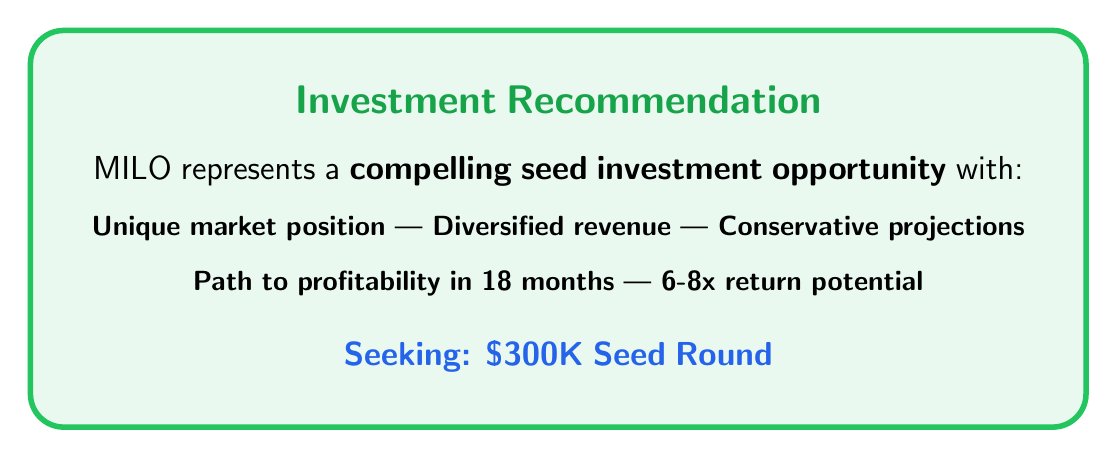
\begin{tikzpicture}
    \node[fill=successgreen!10, draw=successgreen, line width=2pt, rounded corners=12pt,
          inner sep=20pt, text width=12cm, align=center] {
        {\Large\textcolor{darkgreen}{\textbf{Investment Recommendation}}}\\[12pt]
        {\large MILO represents a \textbf{compelling seed investment opportunity} with:}\\[8pt]
        \textbf{Unique market position} | \textbf{Diversified revenue} | \textbf{Conservative projections}\\[8pt]
        \textbf{Path to profitability in 18 months} | \textbf{6-8x return potential}\\[15pt]
        {\large\textcolor{miloprimary}{\textbf{Seeking: \$300K Seed Round}}}
    };
\end{tikzpicture}
\end{center}

\vspace{1.5cm}

% Footer
\begin{center}
    \textcolor{freegray}{\rule{12cm}{0.5pt}}\\[0.4cm]
    \textcolor{freegray}{\small DeepmAInd B.V. | Confidential | Version 3.0 | January 2026}\\[0.2cm]
    \textcolor{freegray}{\scriptsize Conservative projections with realistic growth assumptions}\\
    \textcolor{freegray}{\scriptsize Data sources: Federal Reserve, Veryfi API, Google Gemini, Market Research Reports}
\end{center}

\end{document}
